\section{Устойчивость к шуму и кросс-валидация}
\label{sec:Chapter4}

\subsection{Модели артефактов ЭКГ-сигналов}

В~реальных условиях холтеровского мониторирования запись ЭКГ
неизбежно содержит артефакты различной природы.
В~работе рассматриваются четыре типа помех, наиболее типичных
при~амбулаторной регистрации.

\paragraph{Гауссов шум.}
Моделирует тепловые и~квантовые шумы усилительного тракта:
\begin{equation}
    \tilde{s}[n] = s[n] + \varepsilon[n],\quad
    \varepsilon[n] \sim \mathcal{N}(0,\,\sigma^2).
\end{equation}
Уровень шума характеризуется параметром $\sigma$ и~нарастает
от~$0.01$ до~$0.08$~мВ с~шагом~$0.01$.

\paragraph{Дрейф изолинии.}
Вызван дыхательными движениями и~нестабильным контактом
электрода с~кожей; аппроксимируется медленной синусоидой:
\begin{equation}
    \tilde{s}[n] = s[n] + A\sin\!\left(\frac{2\pi f_0 n}{f_s}\right),
    \quad f_0 = 0.5\;\text{Гц}.
\end{equation}
Амплитуда $A$ варьируется от~$0.01$ до~$0.15$~мВ с~шагом~$0.01$.

\paragraph{Сетевая помеха~50~Гц.}
Индуктивная наводка от~сети электропитания:
\begin{equation}
    \tilde{s}[n] = s[n] + A\sin\!\left(\frac{2\pi \cdot 50 \cdot n}{f_s}\right).
\end{equation}
Амплитуда $A$~--- от~$0.01$ до~$0.08$~мВ.

\paragraph{Мышечный шум~(ЭМГ).}
Сигнал скелетных мышц накладывается на~ЭКГ при~физической
активности; моделируется сглаженным гауссовым шумом:
\begin{equation}
    \tilde{s}[n] = s[n] + (A \cdot \varepsilon) * h[n],
\end{equation}
где $\varepsilon \sim \mathcal{N}(0,1)$, $h[n]$~--- прямоугольный
сглаживающий фильтр длиной~$5$~отсчетов.
Амплитуда $A$~--- от~$0.01$ до~$0.07$~мВ.

\subsection{Результаты экспериментов с шумом}

Для~каждого типа и~уровня помехи вычислялись Accuracy и~Macro~F1
всех~трех моделей на~тестовой выборке~($20\,005$~объектов).
Сводные результаты при~максимальных уровнях помех
приведены в~таблице~\ref{tab:noise_max}.

\begin{table}[h]
\centering
\caption{Метрики при максимальных уровнях шума}
\label{tab:noise_max}
\begin{tabular}{llccc}
\hline
\textbf{Тип шума} & \textbf{Уровень} & \textbf{Модель} &
\textbf{Accuracy} & \textbf{Macro F1} \\
\hline
\multirow{3}{*}{Гауссов шум}      & \multirow{3}{*}{$\sigma{=}0.08$}
  & CNN         & 0.9446 & 0.7869 \\
& & ResNet1D    & 0.8619 & 0.5888 \\
& & RandomForest & \textbf{0.9703} & \textbf{0.8716} \\
\hline
\multirow{3}{*}{Дрейф изолинии}   & \multirow{3}{*}{$A{=}0.15$}
  & CNN         & \textbf{0.9918} & \textbf{0.9740} \\
& & ResNet1D    & 0.9833 & 0.9498 \\
& & RandomForest & 0.9719 & 0.8901 \\
\hline
\multirow{3}{*}{Сетевая помеха}   & \multirow{3}{*}{$A{=}0.08$}
  & CNN         & 0.9832 & 0.9357 \\
& & ResNet1D    & 0.8427 & 0.6395 \\
& & RandomForest & \textbf{0.9767} & \textbf{0.9114} \\
\hline
\multirow{3}{*}{Мышечный шум}     & \multirow{3}{*}{$A{=}0.07$}
  & CNN         & \textbf{0.9882} & \textbf{0.9603} \\
& & ResNet1D    & 0.9758 & 0.9228 \\
& & RandomForest & 0.9830 & 0.9422 \\
\hline
\end{tabular}
\end{table}

\subsubsection{Гауссов шум}

\begin{figure}[h]
\centering
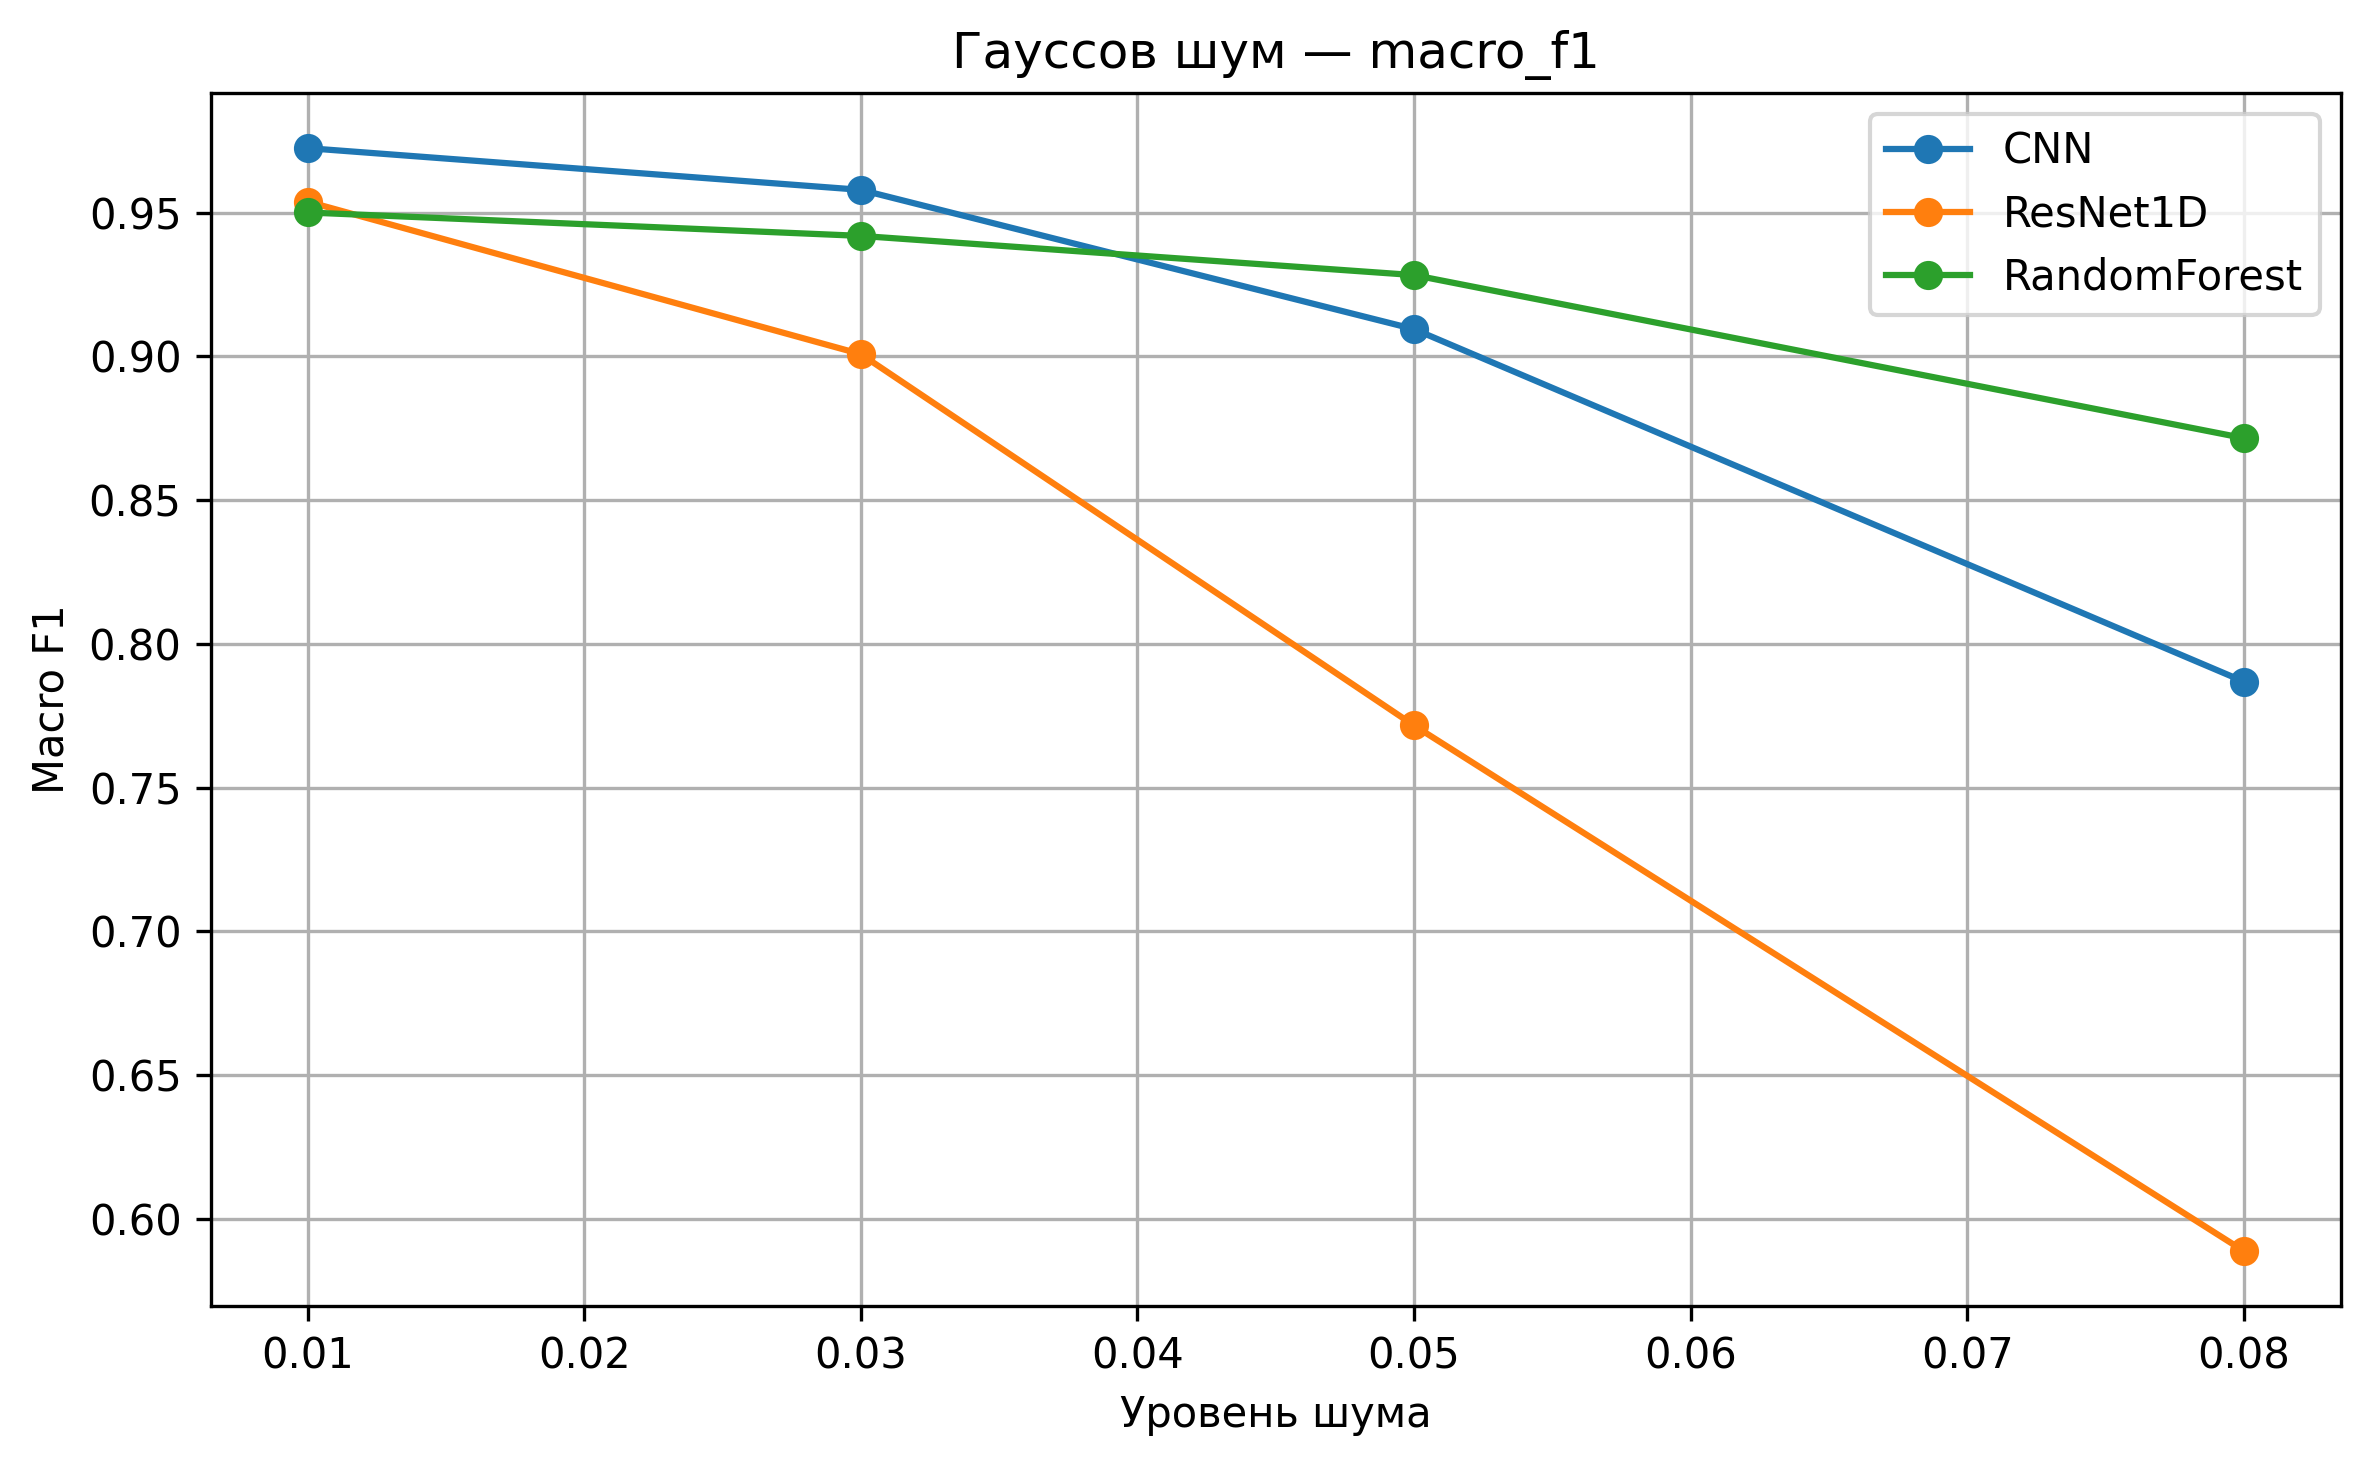
\includegraphics[width=0.85\textwidth]{../reports/figures/models/noise_gaussian_macro_f1.png}
\caption{Зависимость Macro~F1 от~уровня гауссова шума~$\sigma$.}
\label{fig:noise_gaussian}
\end{figure}

При~$\sigma = 0.08$~мВ случайный лес сохраняет Macro~F1~$= 0.872$,
тогда~как~CNN опускается до~$0.787$, а~ResNet1D~--- до~$0.589$.
RF устойчив к~случайным аддитивным помехам: пороговые разбиения
деревьев не~чувствительны к~равномерно распределенному по~спектру
шуму, который усредняется при~нахождении оптимального порога.
CNN теряет точность сильнее: сверточные фильтры обнаруживают
высокочастотные компоненты QRS, которые при~высоком $\sigma$
«маскируются» шумом.

\subsubsection{Дрейф изолинии}

\begin{figure}[h]
\centering
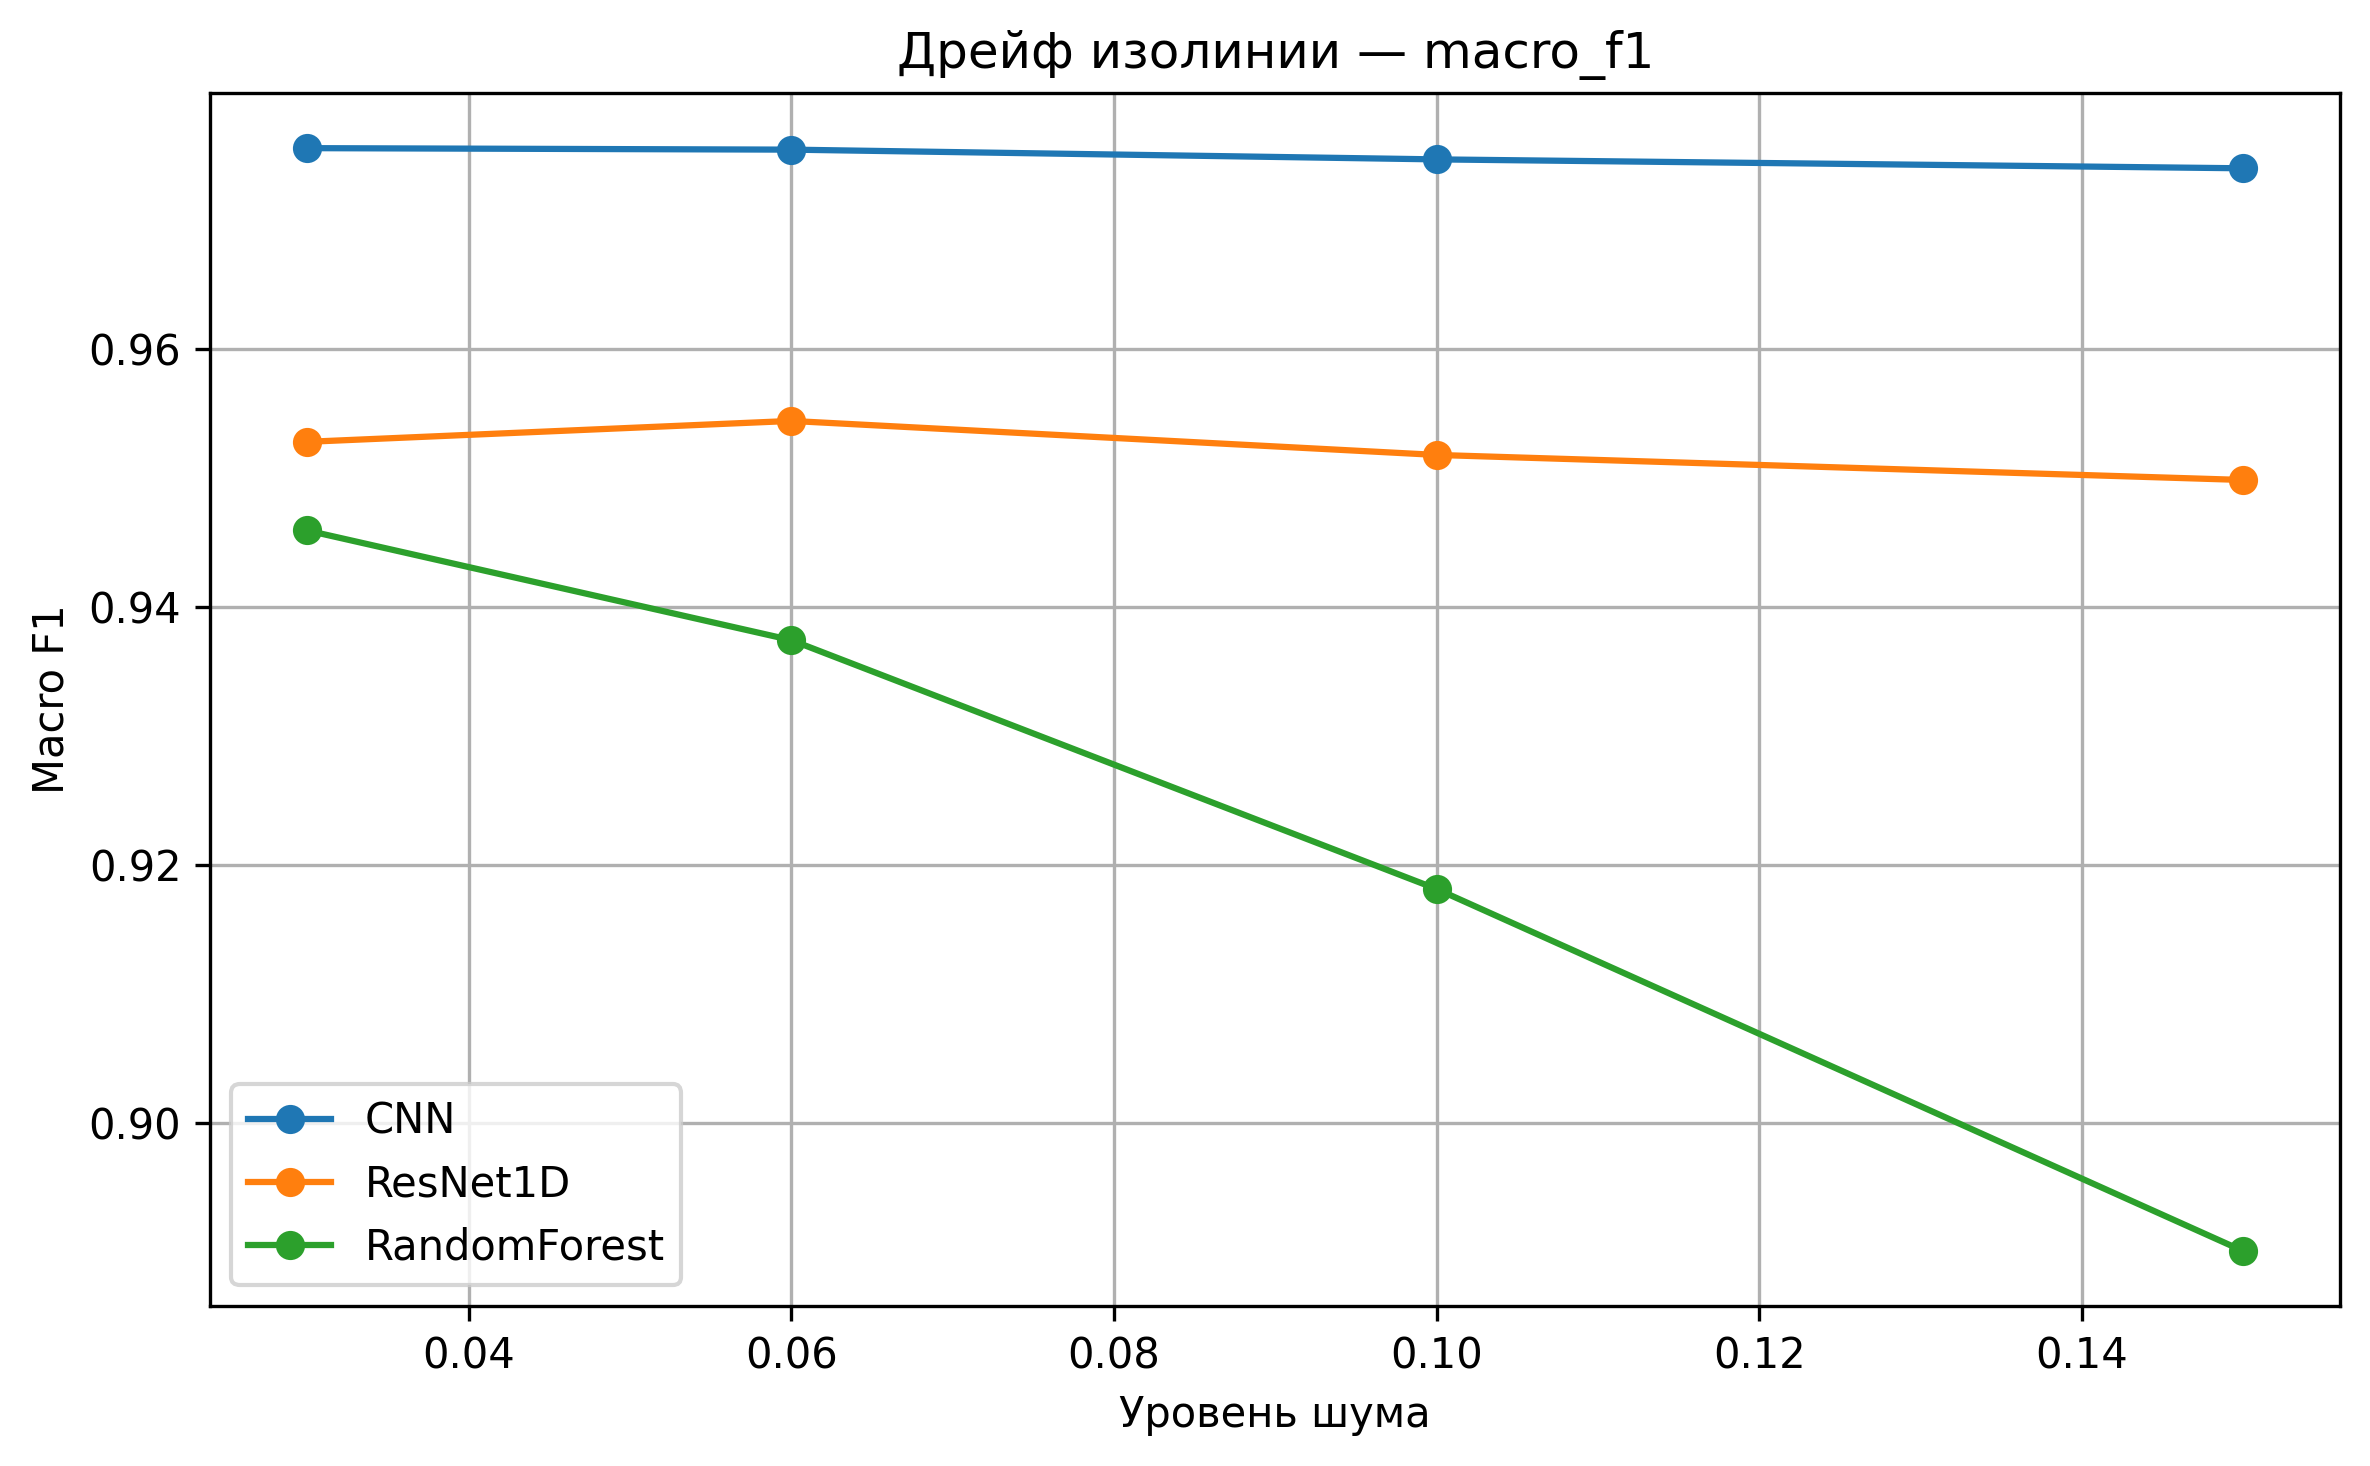
\includegraphics[width=0.85\textwidth]{../reports/figures/models/noise_baseline_macro_f1.png}
\caption{Зависимость Macro~F1 от~амплитуды дрейфа изолинии~$A$.}
\label{fig:noise_baseline}
\end{figure}

Наиболее устойчивой к~дрейфу оказалась CNN:
Macro~F1~$= 0.974$ при~$A = 0.15$~мВ~--- практически без~потерь
относительно чистых данных.
Причина~--- BatchNorm внутри сверточных блоков нормализует
активации по~мини-батчу, фактически компенсируя медленное
смещение изолинии.
ResNet1D также устойчив ($0.950$).
RF деградирует сильнее ($0.890$): деревья строят пороги
по~абсолютным значениям отсчетов и~чувствительны к~сдвигу
постоянной составляющей.

\subsubsection{Сетевая помеха 50~Гц}

\begin{figure}[h]
\centering
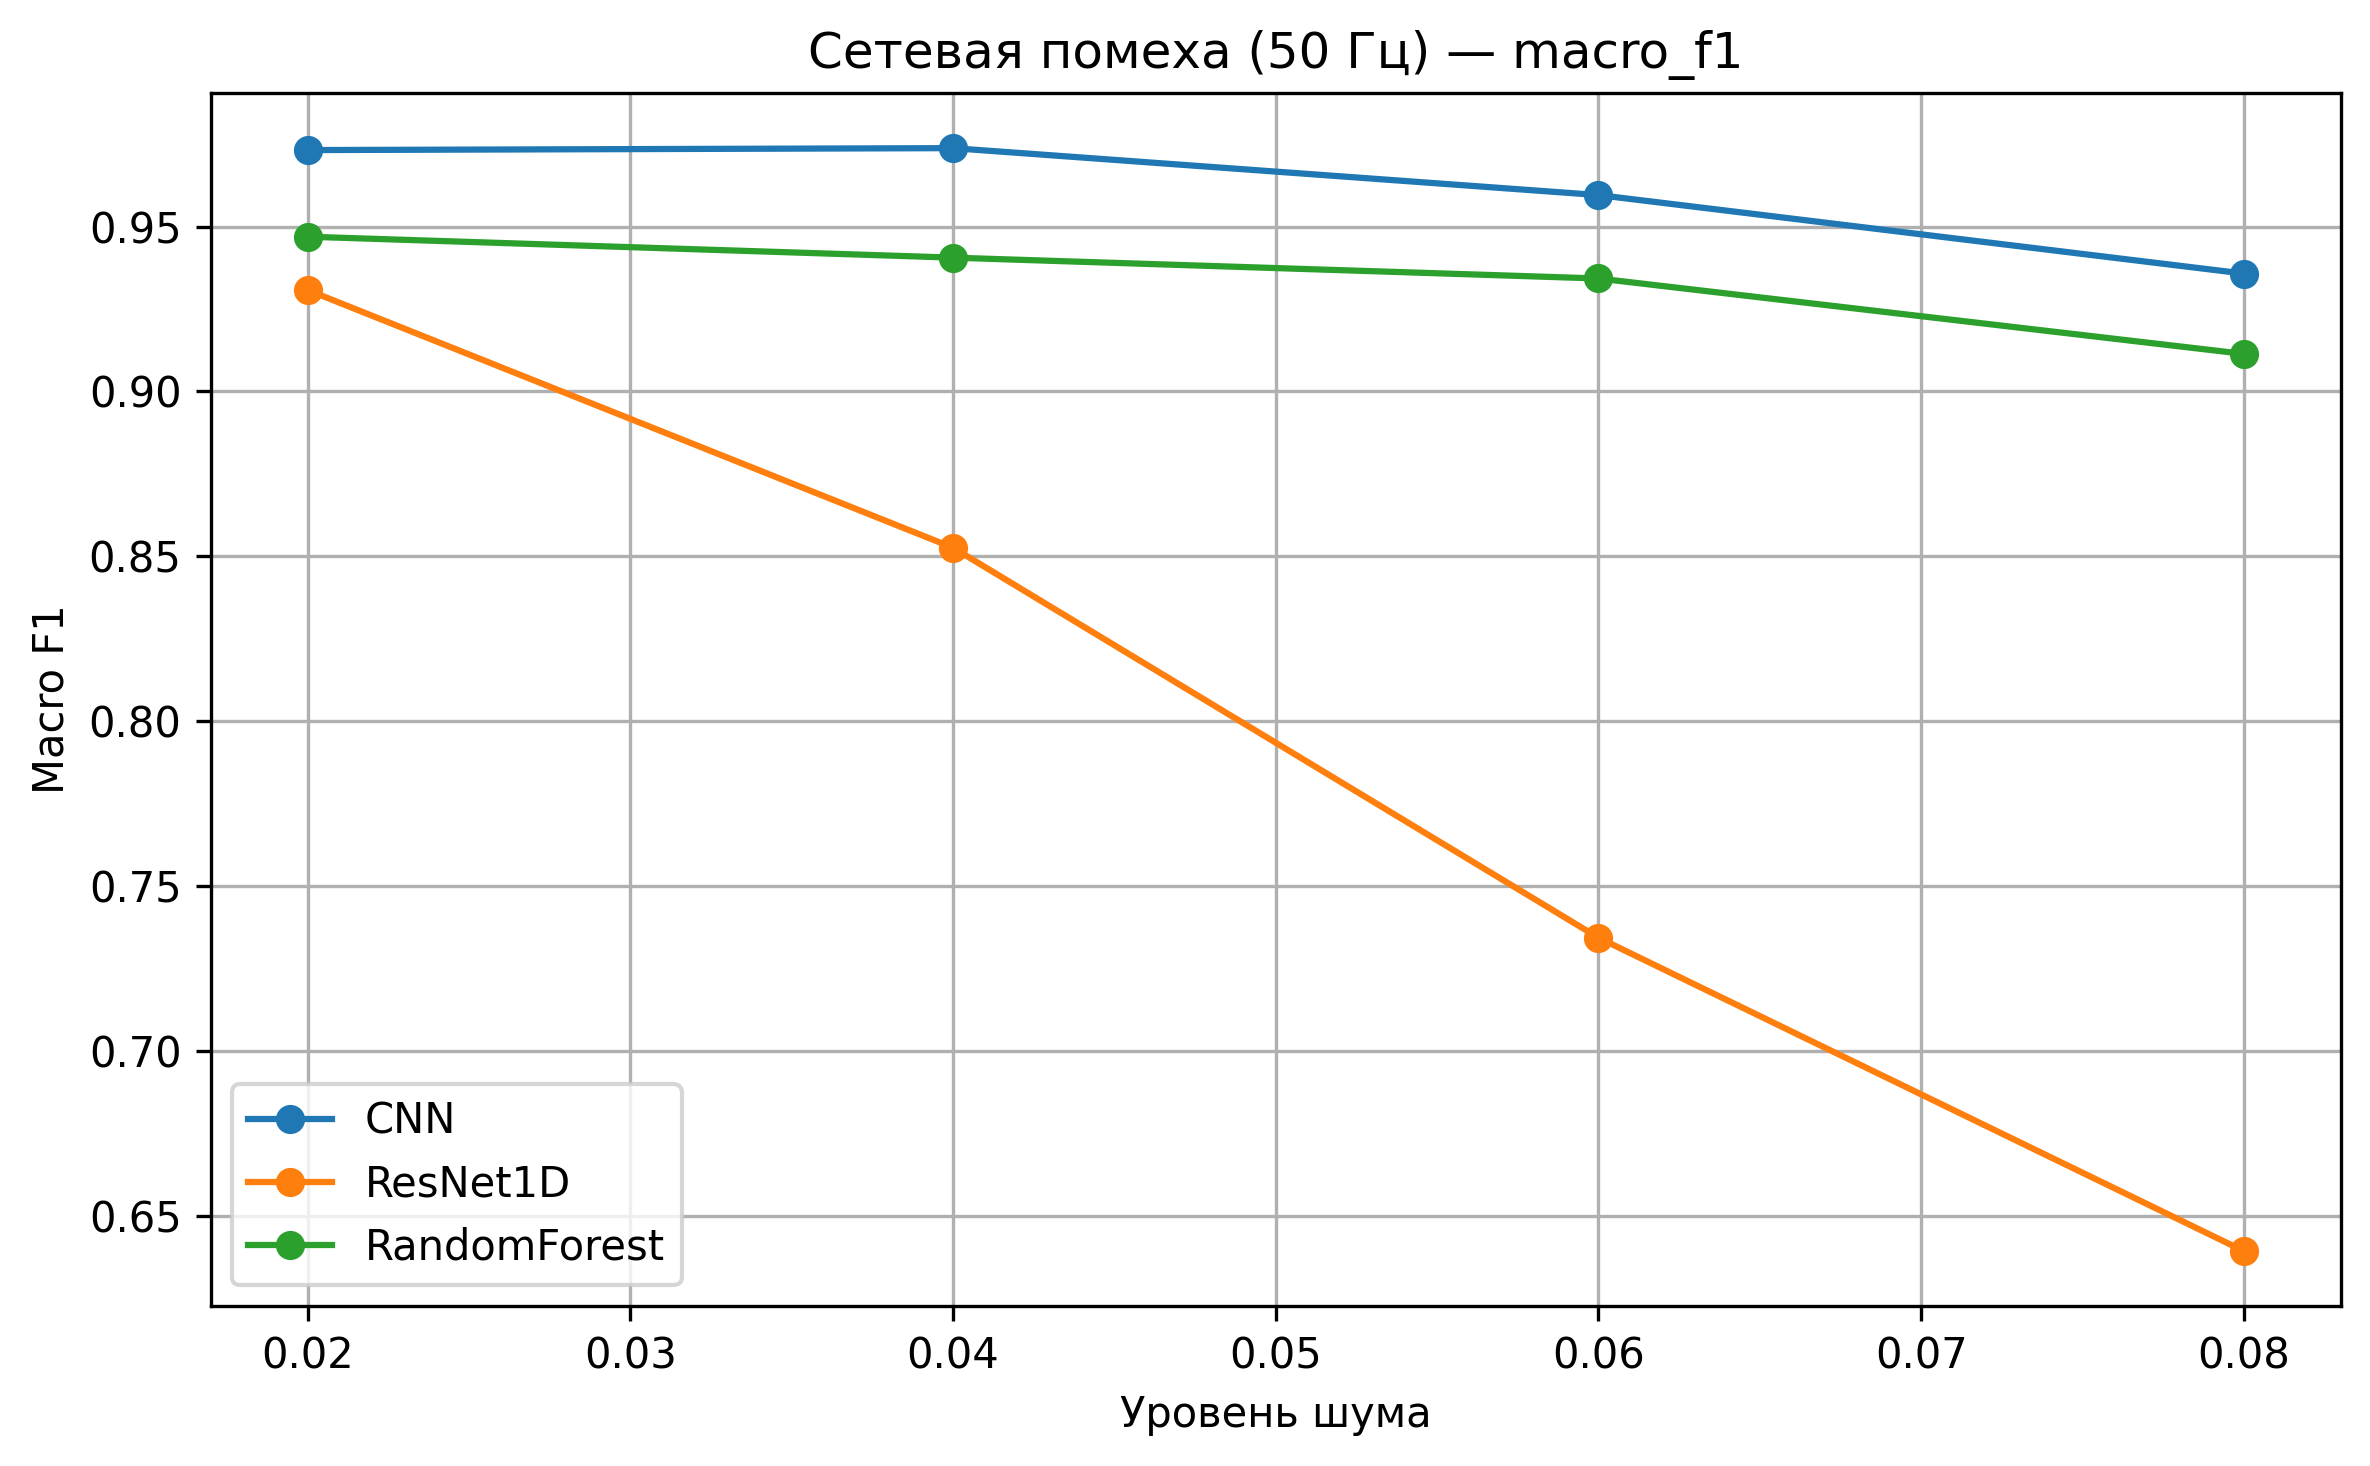
\includegraphics[width=0.85\textwidth]{../reports/figures/models/noise_powerline_macro_f1.png}
\caption{Зависимость Macro~F1 от~амплитуды сетевой помехи~50~Гц.}
\label{fig:noise_powerline}
\end{figure}

Сетевая помеха особенно разрушительна для~ResNet1D:
Macro~F1~падает до~$0.640$~--- потеря $0.31$ относительно
чистых данных.
Слой \texttt{AdaptiveAvgPool1d(1)} глобально усредняет карту
признаков по~временному измерению: периодическая синусоида
частотой~$50$~Гц ($\lambda \approx 7.2$~отсчета) создает
регулярные паттерны, которые после~усреднения дают ненулевые
сдвиги в~признаковом пространстве.
CNN устойчивее ($0.936$): два уровня MaxPool перед
AdaptiveAvgPool частично подавляют высокочастотные компоненты.
RF стабилен ($0.911$): пороговые деления нечувствительны
к~периодическим помехам средней амплитуды.

\subsubsection{Мышечный шум}

\begin{figure}[h]
\centering
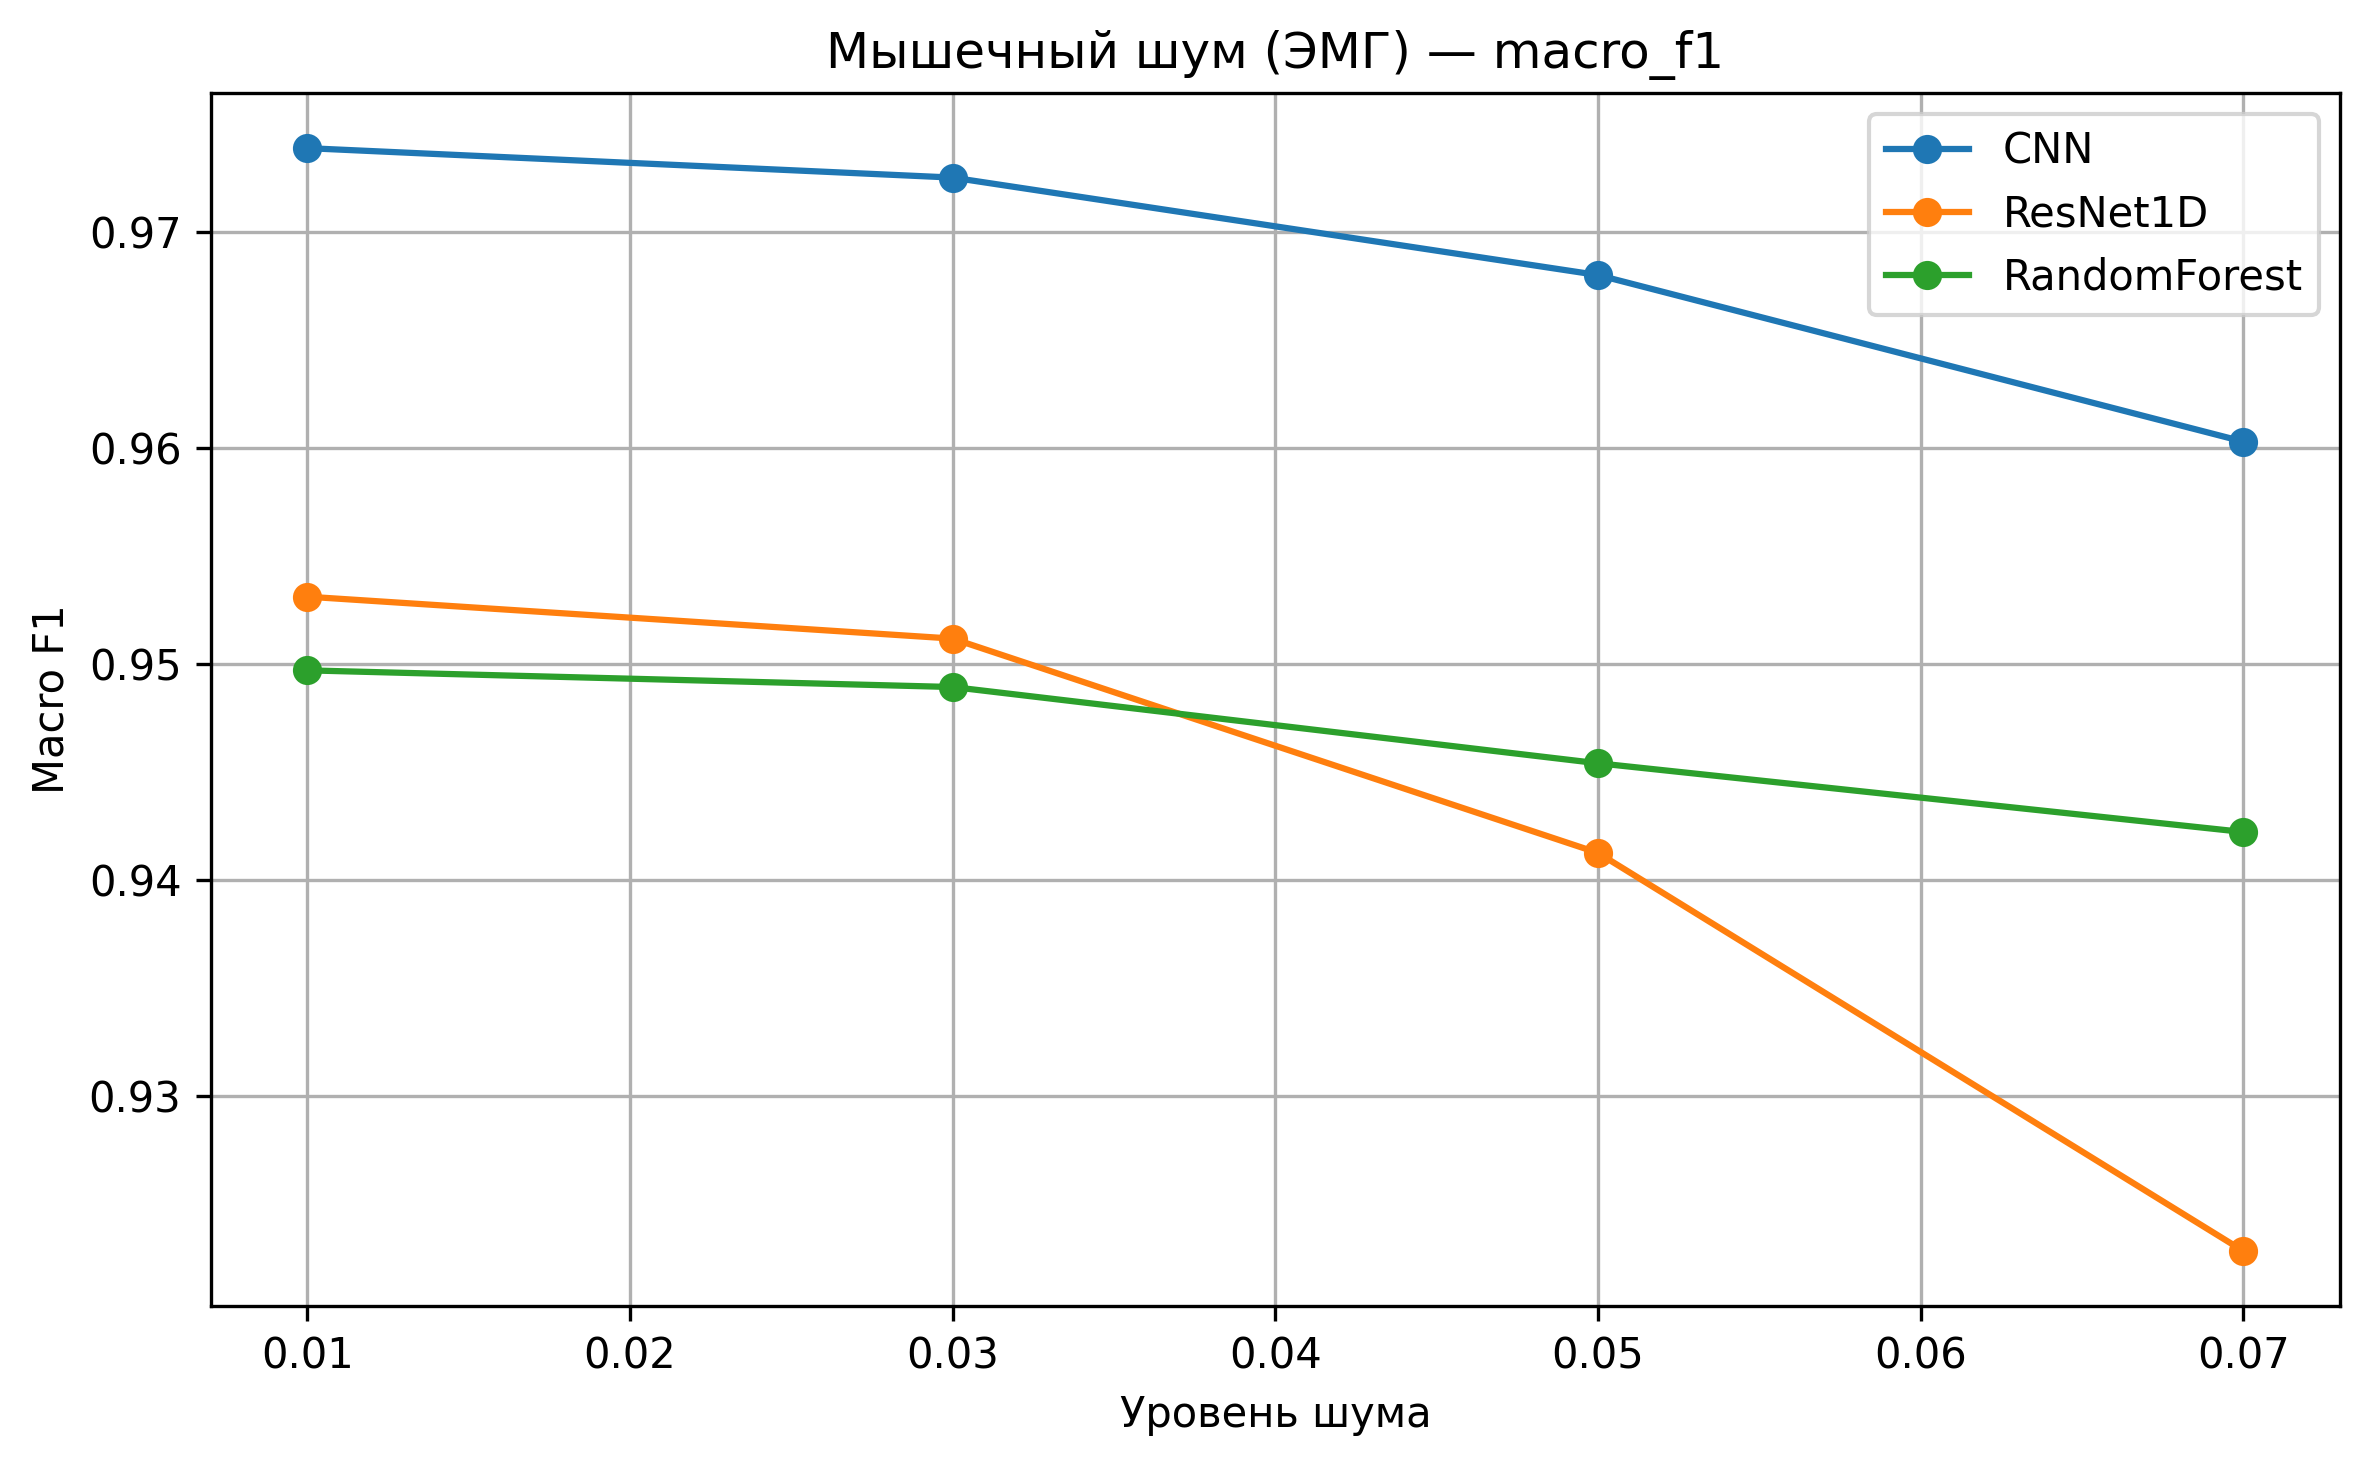
\includegraphics[width=0.85\textwidth]{../reports/figures/models/noise_muscle_macro_f1.png}
\caption{Зависимость Macro~F1 от~амплитуды мышечного шума~$A$.}
\label{fig:noise_muscle}
\end{figure}

Мышечный шум~--- наименее критичная помеха для~всех трех моделей.
CNN лидирует ($0.960$), RF и~ResNet1D показывают близкие результаты
($0.942$ и~$0.923$ соответственно).
Сглаженная структура ЭМГ-шума~(фильтр длиной~$5$~отсчетов)
не~разрушает форму QRS-комплекса~--- именно поэтому
все~модели сохраняют высокое качество.

\subsubsection{Обобщенное сравнение устойчивости}

\begin{figure}[h]
\centering
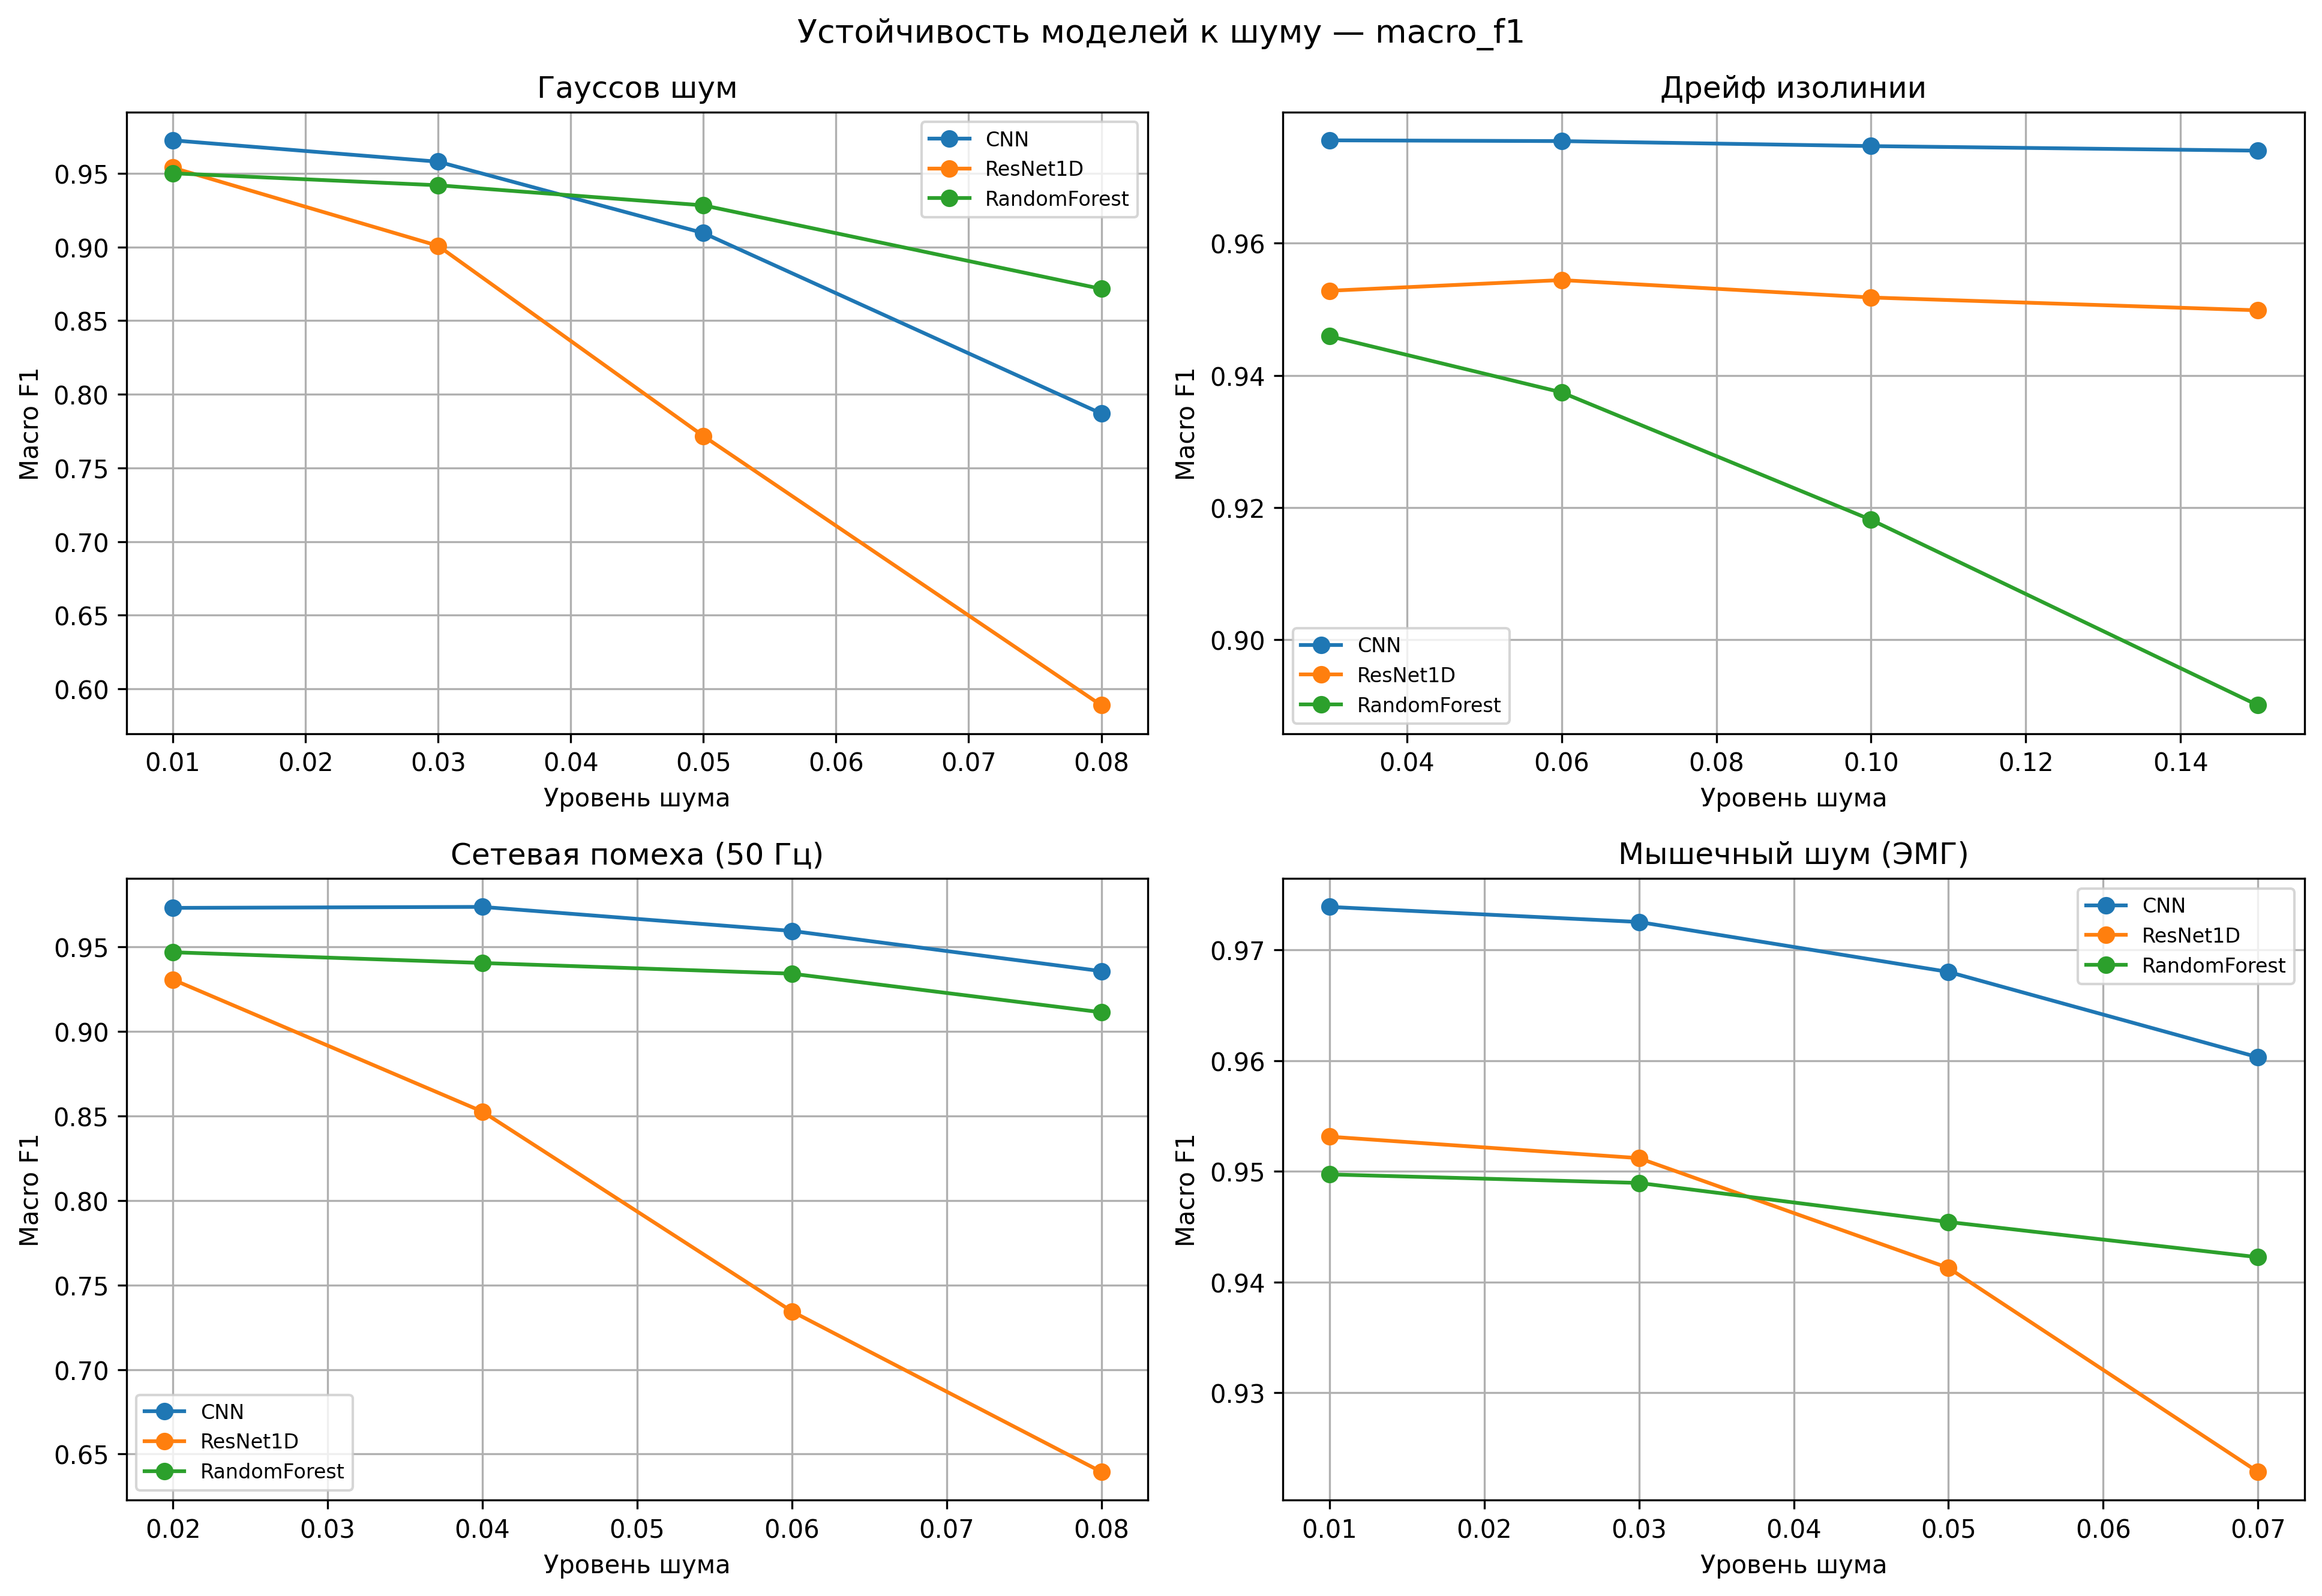
\includegraphics[width=\textwidth]{../reports/figures/models/noise_robustness_macro_f1.png}
\caption{Сводная диаграмма устойчивости: Macro~F1 при~максимальных
уровнях всех четырех типов шума.}
\label{fig:noise_summary}
\end{figure}

Анализ показывает, что~каждая модель имеет свой «профиль
устойчивости»:
\begin{itemize}
    \item \textbf{1D~CNN}~--- лучший выбор при~дрейфе изолинии
    и~мышечном шуме; BatchNorm обеспечивает нечувствительность
    к~медленным трендам.
    \item \textbf{RandomForest}~--- наиболее устойчив к~гауссову
    и~сетевому шуму; пороговая природа деревьев устойчива
    к~равномерным и~периодическим аддитивным помехам.
    \item \textbf{ResNet1D}~--- наименее устойчив в~целом;
    особенно критична сетевая помеха~50~Гц из-за~глобального
    пулинга.
\end{itemize}

\subsection{Кросс-валидация}

\subsubsection{Методология}

Для~оценки стабильности и~обобщающей способности моделей
проводится пятикратная стратифицированная кросс-валидация
($K = 5$).
На~каждой итерации $k$ модель обучается на~$(K-1)/K$ части
данных и~оценивается на~оставшейся $1/K$ части.
Итоговые оценки~--- среднее и~стандартное отклонение
метрик по~фолдам:
\begin{equation}
    \bar{m} \pm \hat{\sigma} = \frac{1}{K}\sum_{k=1}^{K} m_k
    \pm \sqrt{\frac{1}{K-1}\sum_{k=1}^{K}(m_k - \bar{m})^2}.
\end{equation}
Малое~$\hat{\sigma}$ свидетельствует о~стабильности модели
и~отсутствии переобучения на~конкретном разбиении.

\subsubsection{Результаты по фолдам}

Таблица~\ref{tab:cv_folds} содержит значения метрик
для~каждого из~пяти фолдов.

\begin{table}[h]
\centering
\caption{Результаты 5-fold кросс-валидации по фолдам}
\label{tab:cv_folds}
\begin{tabular}{ccccccc}
\hline
\multirow{2}{*}{\textbf{Фолд}} &
\multicolumn{2}{c}{\textbf{RandomForest}} &
\multicolumn{2}{c}{\textbf{CNN}} &
\multicolumn{2}{c}{\textbf{ResNet1D}} \\
& Acc & F1 & Acc & F1 & Acc & F1 \\
\hline
1 & 0.9853 & 0.9528 & 0.9883 & 0.9634 & 0.9378 & 0.8663 \\
2 & 0.9849 & 0.9495 & 0.9800 & 0.9403 & 0.9286 & 0.8553 \\
3 & 0.9851 & 0.9506 & 0.9702 & 0.9185 & 0.7830 & 0.7700 \\
4 & 0.9857 & 0.9533 & 0.9814 & 0.9459 & 0.9709 & 0.9172 \\
5 & 0.9850 & 0.9525 & 0.9898 & 0.9686 & 0.9123 & 0.8391 \\
\hline
\end{tabular}
\end{table}

\subsubsection{Сводные оценки}

\begin{table}[h]
\centering
\caption{Итоговые оценки кросс-валидации (mean\,$\pm$\,std)}
\label{tab:cv_summary}
\begin{tabular}{lcc}
\hline
\textbf{Модель} & \textbf{Accuracy} & \textbf{Macro F1} \\
\hline
RandomForest & $0.9852 \pm 0.0003$ & $\mathbf{0.9517 \pm 0.0016}$ \\
CNN          & $0.9819 \pm 0.0078$ & $0.9473 \pm 0.0199$ \\
ResNet1D     & $0.9065 \pm 0.0723$ & $0.8496 \pm 0.0532$ \\
\hline
\end{tabular}
\end{table}

\begin{figure}[h]
\centering
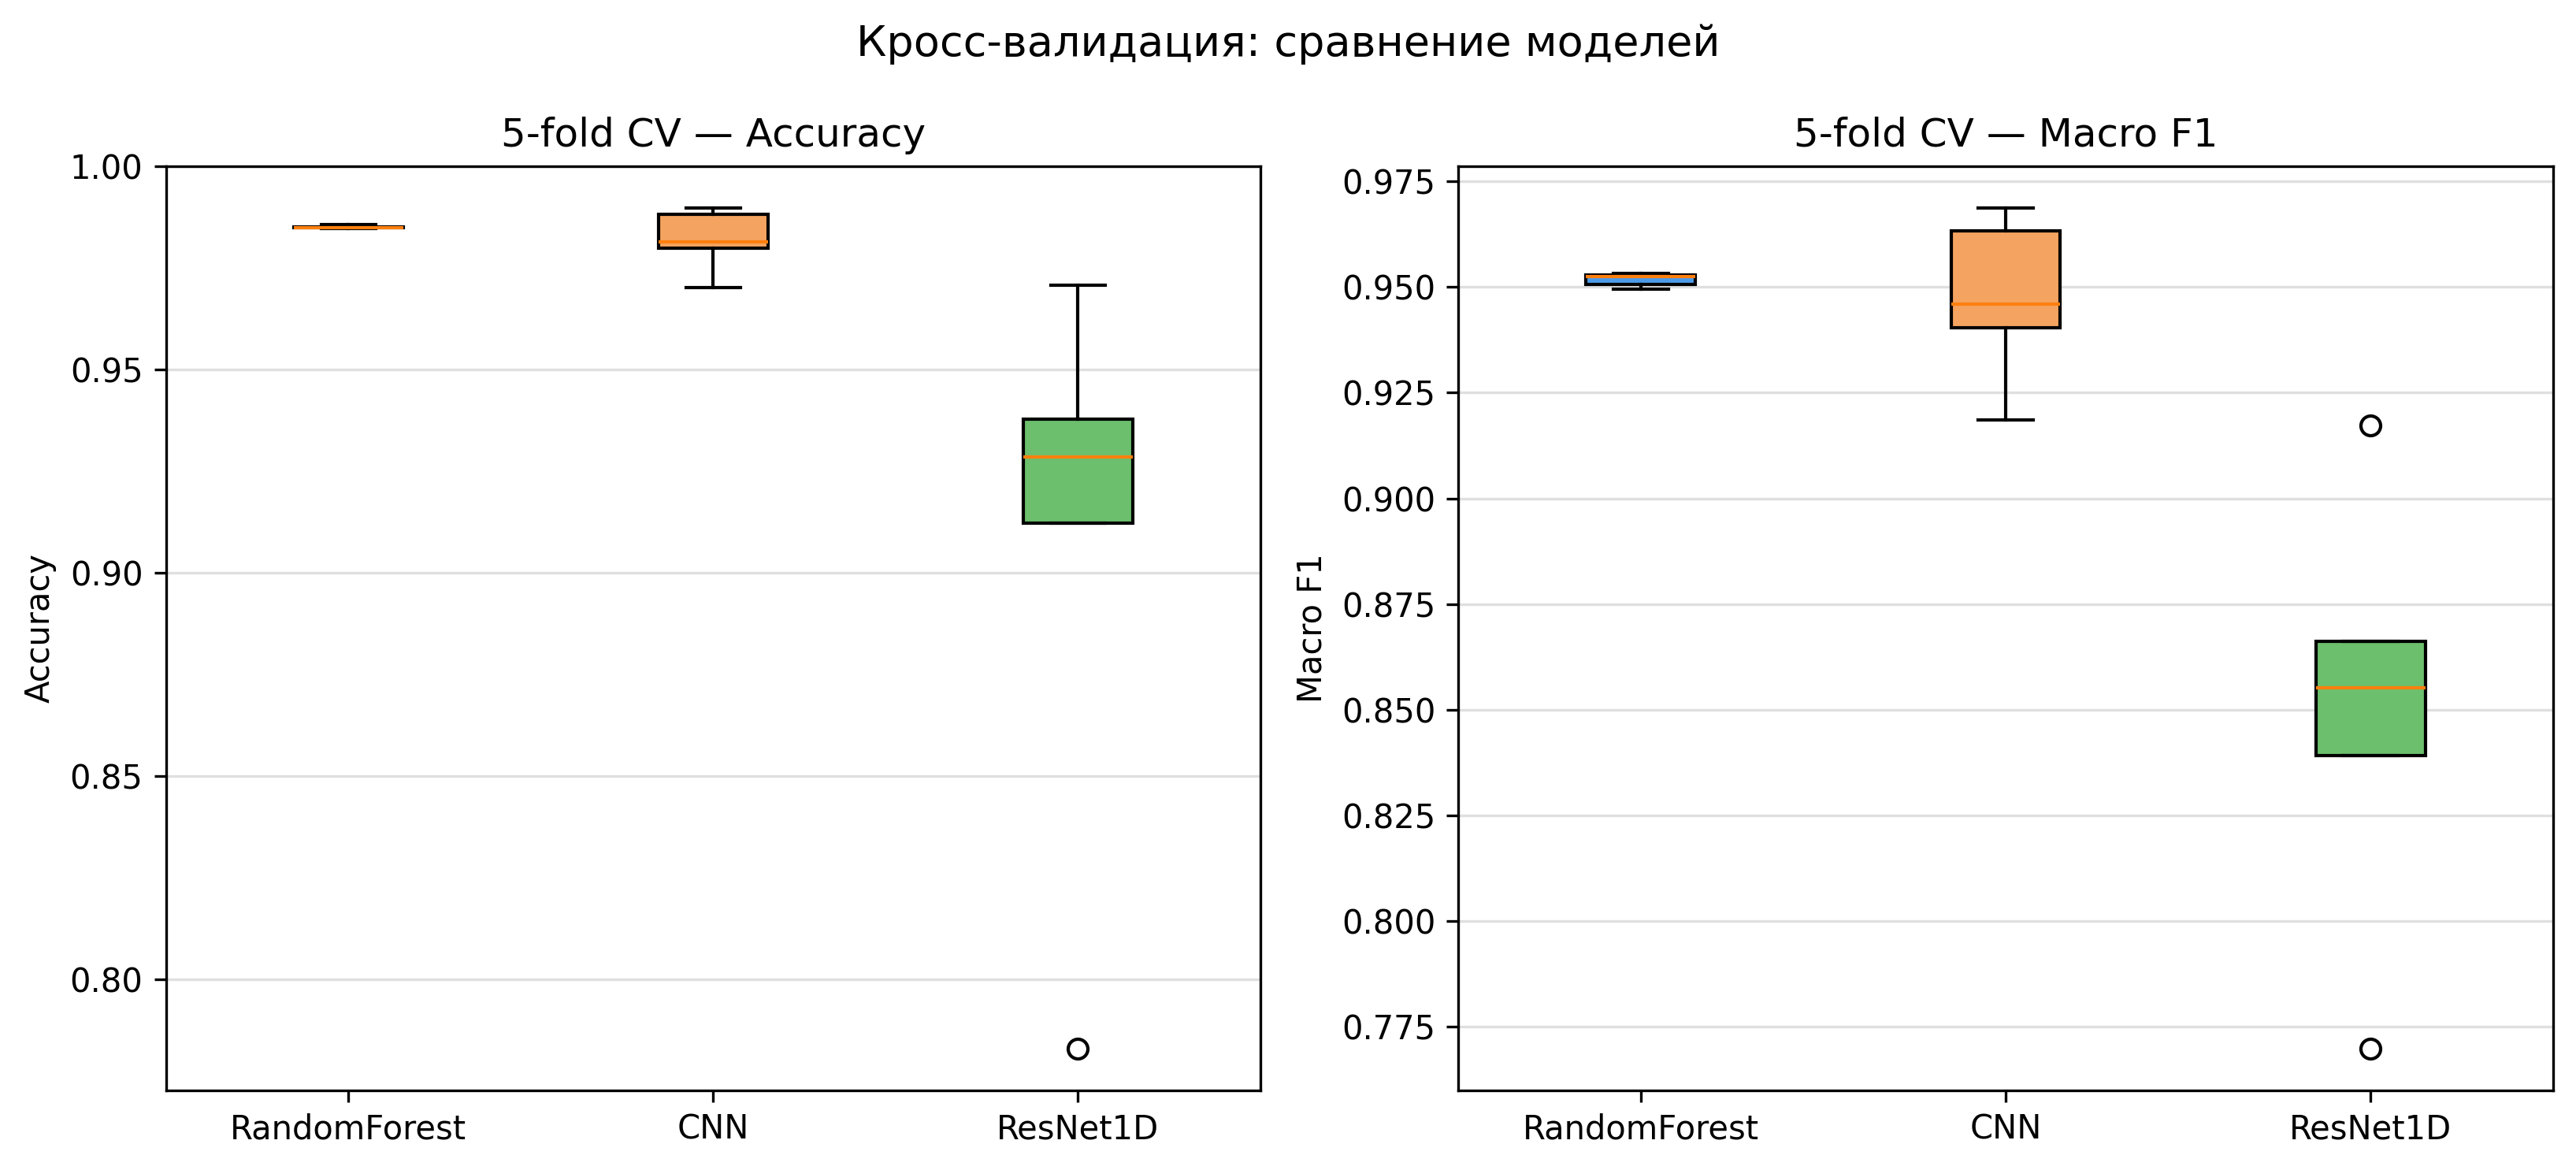
\includegraphics[width=0.85\textwidth]{../reports/figures/models/cv_boxplot.png}
\caption{Box-plot результатов 5-fold кросс-валидации.
Центральная линия~--- медиана, ящик~--- межквартильный диапазон.}
\label{fig:cv_boxplot}
\end{figure}

\subsubsection{Интерпретация}

Результаты кросс-валидации меняют картину относительно
однократного разбиения:

\textbf{Random Forest} демонстрирует наилучшую воспроизводимость:
std Macro~F1~$= 0.0016$~--- почти на~порядок меньше, чем~у~CNN.
Это объясняется тем, что~RF как~ансамблевый метод уже внутренне
усредняет дисперсию за~счет бэггинга и~не~зависит от~случайной
инициализации весов.

\textbf{CNN} при~однократном обучении показывала Macro~F1~$= 0.974$,
однако среднее по~фолдам~$= 0.947 \pm 0.020$~--- ниже RF ($0.952$).
Особенно выбивается \textit{фолд~3}: Macro~F1~$= 0.919$, что~на~$0.028$
ниже медианы.
Это~свидетельствует о~чувствительности нейронной сети
к~распределению данных в~конкретном разбиении.
Вероятная причина~--- в~третьем фолде оказался нетипичный
состав редких классов~(A, V).

\textbf{ResNet1D} показывает наибольшую нестабильность:
std Accuracy~$= 0.072$, std Macro~F1~$= 0.053$.
Критический фолд~3~--- Accuracy~$= 0.783$~--- коллапс
практически до~уровня случайного угадывания для~ряда классов.
Это следствие нехватки эпох~($10$~эпох в~CV против~$30$~при полном
обучении): ResNet1D требует больше итераций для~согласования
остаточных блоков.

\textbf{Вывод}: для~задач, где приоритет~--- воспроизводимость
и~стабильность, RF предпочтительнее нейронных сетей.
Для~достижения максимальной точности при~достаточном объеме
данных и~возможности длительного обучения~--- 1D~CNN.

\subsection{Сопоставление с требованиями постановки задачи}

Таблица~\ref{tab:requirements} содержит итоговую проверку
выполнения требований из~раздела~\ref{sec:Chapter1}.

\begin{table}[h]
\centering
\caption{Выполнение требований постановки задачи}
\label{tab:requirements}
\begin{tabular}{lcccc}
\hline
\textbf{Требование} & \textbf{Порог} & \textbf{RF} & \textbf{CNN} & \textbf{ResNet1D} \\
\hline
Macro F1 (тест)      & $\geq 0.90$ & 0.950~\checkmark & 0.974~\checkmark & 0.953~\checkmark \\
Recall класса A      & $\geq 0.65$ & 0.70~\checkmark  & 0.92~\checkmark  & 0.88~\checkmark  \\
std F1 (CV)          & $\leq 0.03$ & 0.002~\checkmark & 0.020~\checkmark & 0.053~$\times$   \\
Модель сохранена     & ---         & \checkmark       & \checkmark       & \checkmark       \\
\hline
\end{tabular}
\end{table}

RF и~CNN удовлетворяют всем четырем требованиям.
ResNet1D не~выполняет условие на~стабильность (std~$= 0.053 > 0.030$),
что~объясняется недостаточным числом эпох при~кросс-валидации.
При~полном обучении~(30~эпох) ResNet1D стабилен.
